Para alcançar os objetivos propostos no escopo deste trabalho de conclusão de curso, a base de dados a ser utilizada no processo de aprendizado será o conjunto de validação da tarefa \emph{Fine-grained classification} do ILSVRC $2012$ que está disponível em \cite{ref:image-net}. A Figura \ref{fig:visaogeral} apresenta uma visão geral deste conjunto de dados que dispõe de um total de $50$ mil imagens de diferentes naturezas, as quais foram coletadas do \emph{website} Flickr e de outras plataformas semelhantes e rotuladas manualmente por ausência ou presença de $1000$ diferentes categorias \cite{ILSVRC}. 

\begin{figure}[h]
	\centering
	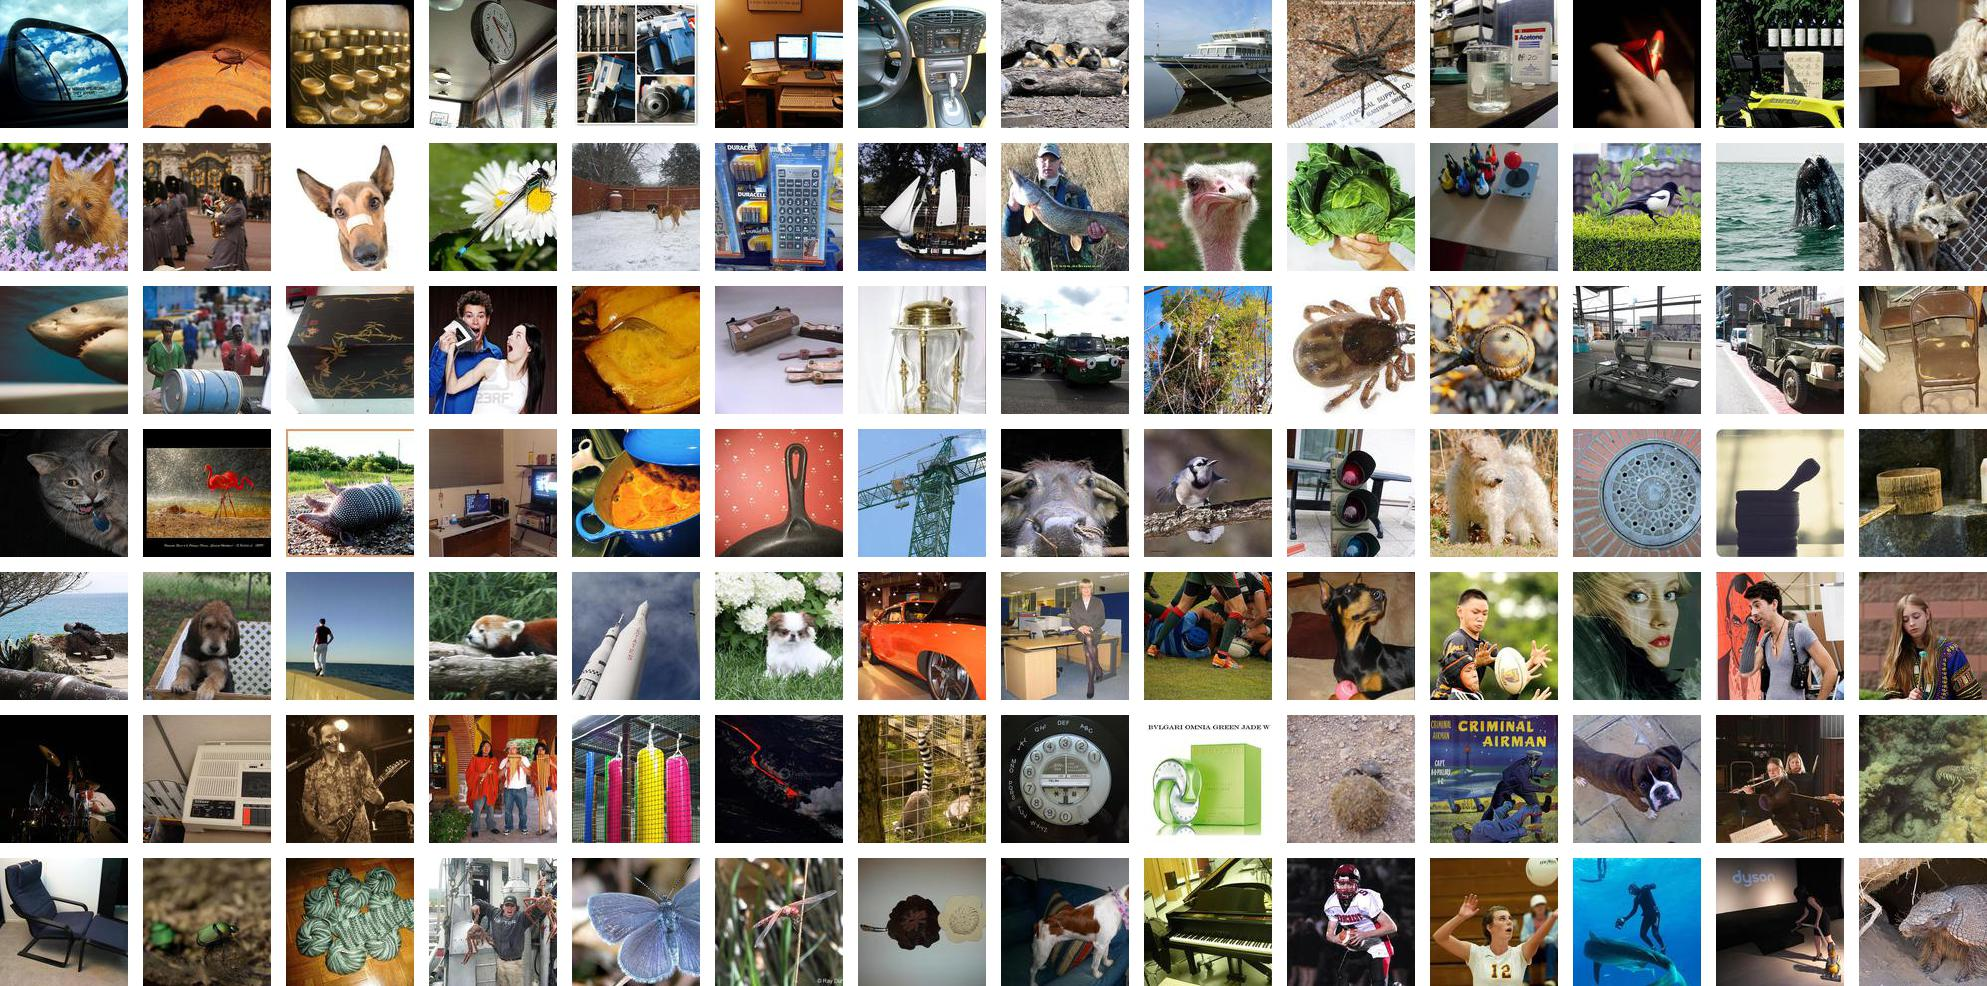
\includegraphics[width=1\textwidth]{./img/visaogeral}
	\caption{Visão geral do conjunto de dados.}
	\label{fig:visaogeral}
\end{figure}

Como dito anteriormente, conjunto de dados será particionado para compor o processo de aprendizado e desse modo $35$ mil imagens serão utilizadas para o treinamento e ajustes dos modelos e as outras $15$ mil para as análises de desempenho. Entretanto, antes de disponibilizar a base de dados para os modelos de DL, as imagens devem estar bem estruturadas e, portanto, devem passar por um pré-processamento, o qual será detalhado na Seção \ref{subsec:pre-process}.

